\documentclass[portrait,final,a0paper,fontscale=0.277]{baposter}

\usepackage{calc}
\usepackage{graphicx}
\usepackage{amsmath}
\usepackage{amssymb}
\usepackage{relsize}
\usepackage{multirow}
\usepackage{rotating}
\usepackage{bm}
\usepackage{url}


\usepackage{scalefnt}

\usepackage{graphicx}
\usepackage{multicol}

%\usepackage{times}
%\usepackage{helvet}
%\usepackage{bookman}
\usepackage{palatino}

\newcommand{\captionfont}{\footnotesize}

\graphicspath{{images/}{../images/}}
\usetikzlibrary{calc}

\newcommand{\SET}[1]  {\ensuremath{\mathcal{#1}}}
\newcommand{\MAT}[1]  {\ensuremath{\boldsymbol{#1}}}
\newcommand{\VEC}[1]  {\ensuremath{\boldsymbol{#1}}}
\newcommand{\Video}{\SET{V}}
\newcommand{\video}{\VEC{f}}
\newcommand{\track}{x}
\newcommand{\Track}{\SET T}
\newcommand{\LMs}{\SET L}
\newcommand{\lm}{l}
\newcommand{\PosE}{\SET P}
\newcommand{\posE}{\VEC p}
\newcommand{\negE}{\VEC n}
\newcommand{\NegE}{\SET N}
\newcommand{\Occluded}{\SET O}
\newcommand{\occluded}{o}

%%%%%%%%%%%%%%%%%%%%%%%%%%%%%%%%%%%%%%%%%%%%%%%%%%%%%%%%%%%%%%%%%%%%%%%%%%%%%%%%
%%%% Some math symbols used in the text
%%%%%%%%%%%%%%%%%%%%%%%%%%%%%%%%%%%%%%%%%%%%%%%%%%%%%%%%%%%%%%%%%%%%%%%%%%%%%%%%

%%%%%%%%%%%%%%%%%%%%%%%%%%%%%%%%%%%%%%%%%%%%%%%%%%%%%%%%%%%%%%%%%%%%%%%%%%%%%%%%
% Multicol Settings
%%%%%%%%%%%%%%%%%%%%%%%%%%%%%%%%%%%%%%%%%%%%%%%%%%%%%%%%%%%%%%%%%%%%%%%%%%%%%%%%
\setlength{\columnsep}{1.5em}
\setlength{\columnseprule}{0mm}

%%%%%%%%%%%%%%%%%%%%%%%%%%%%%%%%%%%%%%%%%%%%%%%%%%%%%%%%%%%%%%%%%%%%%%%%%%%%%%%%
% Save space in lists. Use this after the opening of the list
%%%%%%%%%%%%%%%%%%%%%%%%%%%%%%%%%%%%%%%%%%%%%%%%%%%%%%%%%%%%%%%%%%%%%%%%%%%%%%%%
\newcommand{\compresslist}{%
\setlength{\itemsep}{1pt}%
\setlength{\parskip}{0pt}%
\setlength{\parsep}{0pt}%
}

%%%%%%%%%%%%%%%%%%%%%%%%%%%%%%%%%%%%%%%%%%%%%%%%%%%%%%%%%%%%%%%%%%%%%%%%%%%%%%
%%% Begin of Document
%%%%%%%%%%%%%%%%%%%%%%%%%%%%%%%%%%%%%%%%%%%%%%%%%%%%%%%%%%%%%%%%%%%%%%%%%%%%%%

\begin{document}

%%%%%%%%%%%%%%%%%%%%%%%%%%%%%%%%%%%%%%%%%%%%%%%%%%%%%%%%%%%%%%%%%%%%%%%%%%%%%%
%%% Here starts the poster
%%%---------------------------------------------------------------------------
%%% Format it to your taste with the options
%%%%%%%%%%%%%%%%%%%%%%%%%%%%%%%%%%%%%%%%%%%%%%%%%%%%%%%%%%%%%%%%%%%%%%%%%%%%%%
% Define some colors

%\definecolor{lightblue}{cmyk}{0.83,0.24,0,0.12}
\definecolor{lightblue}{rgb}{0.145,0.6666,1}

% % Draw a video
% \newlength{\FSZ}
% \newcommand{\drawvideo}[3]{% [0 0.25 0.5 0.75 1 1.25 1.5]
%    \noindent\pgfmathsetlength{\FSZ}{\linewidth/#2}
%    \begin{tikzpicture}[outer sep=0pt,inner sep=0pt,x=\FSZ,y=\FSZ]
%    \draw[color=lightblue!50!black] (0,0) node[outer sep=0pt,inner sep=0pt,text width=\linewidth,minimum height=0] (video) {\noindent#3};
%    \path [fill=lightblue!50!black,line width=0pt] 
%      (video.north west) rectangle ([yshift=\FSZ] video.north east) 
%     \foreach \x in {1,2,...,#2} {
%       {[rounded corners=0.6] ($(video.north west)+(-0.7,0.8)+(\x,0)$) rectangle +(0.4,-0.6)}
%     }
% ;
%    \path [fill=lightblue!50!black,line width=0pt] 
%      ([yshift=-1\FSZ] video.south west) rectangle (video.south east) 
%     \foreach \x in {1,2,...,#2} {
%       {[rounded corners=0.6] ($(video.south west)+(-0.7,-0.2)+(\x,0)$) rectangle +(0.4,-0.6)}
%     }
% ;
%    \foreach \x in {1,...,#1} {
%      \draw[color=lightblue!50!black] ([xshift=\x\linewidth/#1] video.north west) -- ([xshift=\x\linewidth/#1] video.south west);
%    }
%    \foreach \x in {0,#1} {
%      \draw[color=lightblue!50!black] ([xshift=\x\linewidth/#1,yshift=1\FSZ] video.north west) -- ([xshift=\x\linewidth/#1,yshift=-1\FSZ] video.south west);
%    }
%    \end{tikzpicture}
% }

\hyphenation{resolution occlusions}
%%
\begin{poster}%
  % Poster Options
  {
  % Show grid to help with alignment
  grid=false,
  % Column spacing
  colspacing=1em,
  % Color style
  bgColorOne=white,
  bgColorTwo=white,
  borderColor=lightblue,
  headerColorOne=black,
  headerColorTwo=lightblue,
  headerFontColor=white,
  boxColorOne=white,
  boxColorTwo=lightblue,
  % Format of textbox
  textborder=roundedleft,
  % Format of text header
  %eyecatcher=true,
  eyecatcher=true,
  headerborder=closed,
  headerheight=0.1\textheight,
%  textfont=\sc, An example of changing the text font
  headershape=roundedright,
  headershade=shadelr,
  headerfont=\Large\bf\textsc, %Sans Serif
  textfont={\setlength{\parindent}{1.5em}},
  boxshade=plain,
%  background=shade-tb,
  background=plain,
  linewidth=2pt
  }
  % Eye Catcher
  {%
\includegraphics[height=1.0em]{images/CodeCogsEqn.pdf}
  
\includegraphics[height=8.5em]{images/zimt_logo_square_RGB-1024x738.png}
  } 
  % Title
  {\begingroup
    \scalefont{1.0}
      \bf\textsc{Ithaka: a taxonomic classifier \\
      {\vspace{-0.2em} \scalefont{0.7} based on \\} 
      \vspace{0.0em}	
            Bloom filters, and spaced seeds}
   \endgroup
   \vspace{0.06em}}
  % Authors
  {\textsc{Maciej Sykulski, Karel B{\v r}inda, Gregory Kucherov}\\
   {\small macieksk@gmail.com, karel.brinda@univ-mlv.fr, gregory.kucherov@univ-mlv.fr}
   }   
      %\{ Brian.Amberg and Thomas.Vetter \}@unibas.ch}}
  % University logo
  {% The makebox allows the title to flow into the logo, this is a hack because of the L shaped logo.
    
    
\includegraphics[height=8.0em]{images/UPEM_LOGO_SIGNALETIQUE_SMALL.pdf}
  }

%%%%%%%%%%%%%%%%%%%%%%%%%%%%%%%%%%%%%%%%%%%%%%%%%%%%%%%%%%%%%%%%%%%%%%%%%%%%%%
%%% Now define the boxes that make up the poster
%%%---------------------------------------------------------------------------
%%% Each box has a name and can be placed absolutely or relatively.
%%% The only inconvenience is that you can only specify a relative position 
%%% towards an already declared box. So if you have a box attached to the 
%%% bottom, one to the top and a third one which should be in between, you 
%%% have to specify the top and bottom boxes before you specify the middle 
%%% box.
%%%%%%%%%%%%%%%%%%%%%%%%%%%%%%%%%%%%%%%%%%%%%%%%%%%%%%%%%%%%%%%%%%%%%%%%%%%%%%
    %
    % A coloured circle useful as a bullet with an adjustably strong filling
    \newcommand{\colouredcircle}{%
      \tikz{\useasboundingbox (-0.2em,-0.32em) rectangle(0.2em,0.32em); \draw[draw=black,fill=lightblue,line width=0.03em] (0,0) circle(0.18em);}}

%%%%%%%%%%%%%%%%%%%%%%%%%%%%%%%%%%%%%%%%%%%%%%%%%%%%%%%%%%%%%%%%%%%%%%%%%%%%%%
  \headerbox{Metagenomics \& NGS}{name=problem,column=0,row=0}{
%%%%%%%%%%%%%%%%%%%%%%%%%%%%%%%%%%%%%%%%%%%%%%%%%%%%%%%%%%%%%%%%%%%%%%%%%%%%%%

Metagenomics is a powerful approach to study genetic material contained
in environmental samples, which is revolutionized by high-throughput sequencing
technologies. Taxonomic classification of metagenomics data sets is a common step in analysis, a step for which computational cost becomes prohibitive with the growth of metagenomic datasets.

Approaches using sequence alignment algorithms, often based on the Burrows-Wheeler transform, such as Kaiju\cite{kaiju}, Centrifuge\cite{centrifuge}, compete successfully with k-mer based alignment-free comparison methods such as Kraken\cite{kraken}, Clark\cite{clark}. Improvements to k-mer based approaches include: extending contiguous k-mers with spaced seeds \cite{sseed}\cite{clark}, using Bloom filters as an underlying data structure for storing k-mers.\cite{trie}

%     {\bf Metagenomics} is a powerful approach to study genetic
% content of environmental samples, which has been strongly promoted
% by NGS technologies.
% %
% 
% For large-scale metagenomic projects
% %, alignment-based approaches appear unfeasible, and 
% alignment-free methods are used.
% %aligning multimillion read sets against thousands
% %of genomes remains computationally difficult even with optimized
% %tools. 
% %
% To cope with massive data,
% %involved in modern metagenomic projects, 
% recent tools 
% %(Ames et al., 2013; Wood and
% %Salzberg, 2014) 
% (LMAT \cite{lmat}, Kraken \cite{kraken})
% rely on the analysis of {\bf k-mers} (words of fixed size)
% shared between the
% {\bf read} to be classified, and {\bf reference genomes}.

   \vspace{0.3em}
 }



%%%%%%%%%%%%%%%%%%%%%%%%%%%%%%%%%%%%%%%%%%%%%%%%%%%%%%%%%%%%%%%%%%%%%%%%%%%%%%
  \headerbox{References}{name=references,column=0,above=bottom}{
%%%%%%%%%%%%%%%%%%%%%%%%%%%%%%%%%%%%%%%%%%%%%%%%%%%%%%%%%%%%%%%%%%%%%%%%%%%%%%
    \smaller
    \bibliographystyle{ieee}
    \renewcommand{\section}[2]{\vskip 0.05em}
      \begin{thebibliography}{1}\itemsep=-0.01em
      \setlength{\baselineskip}{0.4em}
%       \bibitem{noe:coverage}
%          L.~No{\'e}, D.~E.~K.~Martin.
%          \newblock {A} coverage criterion for spaced seeds and its
%         applications to support vector machine string kernels and k-mer
%       distances. 
%       \newblock In Journal of Computational Biology 21, 2014.
%       %      
\bibitem{kaiju} %[1]
Menzel,~P, Ng~Kim~Lee, Krogh~A
\newblock Fast and sensitive taxonomic classification for metagenomics with Kaiju.
\newblock Nat Commun 7, Nature Publishing Group, apr 2016, 
      
\bibitem{centrifuge} Kim~D, Song~L, Breitwieser~F~P, Salzberg~S %[2]
\newblock Centrifuge: rapid and sensitive classification of metagenomic sequences
\newblock Genome 1.2: 2.

\bibitem{kraken} %[3]
      Wood,~D.~E. and Salzberg,~S.~L.
      \newblock Kraken: ultrafast metagenomic sequence classification using exact alignments. 
      \newblock In Genome Biol., 15(3), R46. (2014)

\bibitem{clark} Ounit~R, Lonardi~S, %[4,6]
\newblock Higher classification sensitivity of short metagenomic reads with CLARK-S
\newblock bioRxiv 053462; doi: http://dx.doi.org/10.1101/053462

\bibitem{sseed} Břinda,~K,Sykulski~M, Kucherov~G.  %[5]
\newblock Spaced seeds improve k-mer-based metagenomic classification.
\newblock Bioinformatics 31.22 (2015): 3584-3592.

\bibitem{trie} Holley~G, Wittler~R, Stoye~J.  %[7]
\newblock Bloom Filter Trie: an alignment-free and reference-free data structure for pan-genome storage. 
\newblock Algorithms for Molecular Biology. 2016;11: 3.      
            
      \end{thebibliography}

 \hspace{-2.0em}
  \begin{minipage}{\textwidth}
  \begin{minipage}{0.80\linewidth}
  %  \indent{}
  %The source code \\ and the manual \\ are available at   
   {\smaller 
  \url{https://github.com/gregorykucherov/ithaka}\\
  \url{http://seed-kraken.readthedocs.org} 
  %\url{http://arxiv.org/abs/1502.06256}
   }
  \end{minipage}\hfill%
  \begin{minipage}{0.20\linewidth}
  %\hfill
\includegraphics[width=\linewidth]{images/qr-seed-kraken-rea-crop.pdf}
  \hfill
\includegraphics[width=\linewidth]{images/qrcode-ithaka.png}
  \end{minipage}
  \end{minipage}
   \vspace{0.3em}
  }



%%%%%%%%%%%%%%%%%%%%%%%%%%%%%%%%%%%%%%%%%%%%%%%%%%%%%%%%%%%%%%%%%%%%%%%%%%%%%%
  \headerbox{Spaced Seeds}{name=method,column=0,below=problem}{
%%%%%%%%%%%%%%%%%%%%%%%%%%%%%%%%%%%%%%%%%%%%%%%%%%%%%%%%%%%%%%%%%%%%%%%%%%%%%%

  A {\bf spaced seed} is a pattern over alphabet 
  $A=\{\textbf{\#}, \textbf{--}\}$, where\\
  $\#$ matching position,\, $-$ don't care position.
\vspace{-0.5em}  
  \noindent{\begin{center}
	    
\includegraphics[height=2.5em]{images/CodeCogsEqn.pdf}
	    %{images/seed_expl-crop.pdf}
	    \end{center}}
\vspace{-0.8em}
A seed acts as a mask for comparing short oligonucleotides.
The number of $\textbf{\#}$'s in a seed, called {\em weight},
defines the number k of matching nucleotides. 
In the above example k = 4, seed span = 6,
and the matching (spaced) k-mer is ${\bf ACTC}$ signifying a {\bf hit}.

A {\bf coverage} is a number of aligned pairs covered 
by $\textbf{\#}$ from a spaced seed matches while sliding over an alignment 
(=4 above).
   \vspace{0.3em}
  }

% 
% %%%%%%%%%%%%%%%%%%%%%%%%%%%%%%%%%%%%%%%%%%%%%%%%%%%%%%%%%%%%%%%%%%%%%%%%%%%%%%
%   \headerbox{Contributions}{name=contribution,column=0,below=method, above=references}{
% %%%%%%%%%%%%%%%%%%%%%%%%%%%%%%%%%%%%%%%%%%%%%%%%%%%%%%%%%%%%%%%%%%%%%%%%%%%%%%
% %\begin{itemize}
% $\bullet$\,We showed that spaced seeds can improve success
%   rate of binary classification of alignments into two categories, each
%   defined by a specific mismatch rate.
%   %Here the classification is done
%   %through ``querying'' an alignment using a seed as a mask and
%   %reporting whether the seed applies at a given position. 
%   For example,
%   in discriminating between alignments of length 100 with mismatch
%   rate $0.2$ and $0.3$, a spaced seed of weight 16 achieves 63\% of
%   success while a contiguous seed of the same weight achieves only
%   40\%. 
% 
% $\bullet$\,We demonstrated that spaced seeds allow for a better
%   classification of NGS reads coming from a genome $G$ between two
%   other genomes $G_1$ and $G_2$ of the same genus. 
%   %Here reads are
%   %classified according to the phylogenetic distance
%   %between $G$ and $G_1$ and $G$ and $G_2$ respectively. We established that correct classification is obtained
%   %with seeds of weight 16 and more, while seeds of weight 14 are
%   %insufficient. 
% 
% $\bullet$\,We analyzed how well different estimators (coverage/hit-number
%   combined with spaced/contiguous seed) correlate with the alignment
%   quality, also on real genomes. %(center panel).
%   %, by measuring Spearman's rank correlation
%   %coefficient and mutual information coefficient.
%     
% %$\bullet$\,We compare spaced and contiguous seeds through
% % large-scale metagenomics experiments (right panel).
% $\bullet$\,We demonstrated that spaced seeds can improve the sensitivity-selectivity trade-off in large-scale metagenomics experiments ({\sc seed-Kraken} panel).
% %
% %\noindent{\bf Results:}
% %     Within this general framework, we show that spaced
% % seeds provide a significant improvement of classification capacity as
% % opposed to traditional contiguous k-mers. We support this thesis
% % through a series a different computational experiments, including
% % simulations of large-scale metagenomic projects.
%    
% % %To study this, we implemented the
% % %following experimental setup. 
% % %
% % Using {\sc dwgsim} read simulator
% % %(\url{http://github.com/nh13/DWGSIM}), 
% % we generate single-end
% % {\sc Illumina}-like reads from genome $G$. 
% % %In all experiments, 
% % We assumed
% % 1\% of base mutations (substitutions only), and 2\% of sequencing
% % errors. 
% % %({\sc dwgsim} options \texttt{-e 0.02 -r 0.01 -R 0}). 
% % Given a seed  $k$-mers of $G_1$ and $G_2$ are indexed.
% % %to support existence queries only. 
% % For each read, all $k$-mers are
% % queried against $G_1$ and $G_2$ and corresponding counts $C_1$ and
% % $C_2$ are computed. If $C_1>C_2$ (resp. $C_1<C_2$), the read is classified to be closer
% % to $G_1$ (resp. $G_2$), otherwise a tie is reported. 
% % 
% % {\noindent
% % \scriptsize 
% % % \begin{table}
% \caption{\small Classification of {\em Bacillus thuringiensis} reads
%   against {\em Bacillus anthracis} and {\em Bacillus cereus} genomes. Each entry contains a pair ``Fraction (in \%) of reads
%   classified closer to {\em B.anthracis}\, /\,Fraction of reads
%   classified closer to {\em B.cereus} ''. Spaced seeds used are
%   shown in Table~\ref{smeg_gil_van}.\label{thur_anth_cer}}
% \centering
\begin{tabular}{|r|c|c|c|c|}%c|}
\hline
& \multicolumn{4}{c|}{weight}\\
\cline{2-5}
                        & 14            & 16         & 18        & 20       
                        \\%& 22\\
                        
\hline
  contig hit nb    & 83 / 14 & 81 / 11 & 79 / 09 & 77 / 08 \\%& 76 / 08\\
  contig cover     & 78 / 17 & 80 / 12 & 79 / 09 & 77 / 08 \\%& 76 / 08\\
\hline
  spaced hit nb    & 83 / 13 & 82 / 11 & 80 / 09 & 79 / 09 \\%& 79 / 08\\
  spaced cover    & 80 / 15 & 81 / 11 & 80 / 09 & 79 / 09 \\%& 79 / 08\\
\hline
\end{tabular}
% \end{table}


% % }  
% % \vspace{0.3em}
% % % \caption{\small 
% % Classification of {\em Bacillus thuringiensis} reads
% %   against {\em Bacillus anthracis} and {\em Bacillus cereus} genomes. Each entry contains a pair ``Fraction (in \%) of reads
% %   classified closer to {\em B.anthracis}\, /\,Fraction of reads
% %   classified closer to {\em B.cereus} ''.
% % %
% \vspace{0.3em}
%   }


%%%%%%%%%%%%%%%%%%%%%%%%%%%%%%%%%%%%%%%%%%%%%%%%%%%%%%%%%%%%%%%%%%%%%%%%%%%%%%
\headerbox{Scores on real genomes}{name=results,column=1,span=1,row=0}{
  %%%%%%%%%%%%%%%%%%%%%%%%%%%%%%%%%%%%%%%%%%%%%%%%%%%%%%%%%%%%%%%%%%%%%%%%%%%%%%
%For a given genome $G$
We generated a set of {\sc Illumina}-like single-end reads:
we've selected random substrings of 
{\em M.tuberculosis} genome
%$G$
of length $L=100$ and
introduced $k$ mismatch errors, with $k$ random between $1$ and $20$.
For each read, we computed: {\bf number of hits} and {\bf coverage}
to the genome under a given seed.
%This experiment has been applied to {\em M. tuberculosis} genome, 
A typical plot error vs score (seed weight 20).
\noindent\begin{tabular}{@{\hspace{0.0em}}c@{\hspace{0.0em}}c@{\hspace{0.0em}}}
Hits & Coverage\\
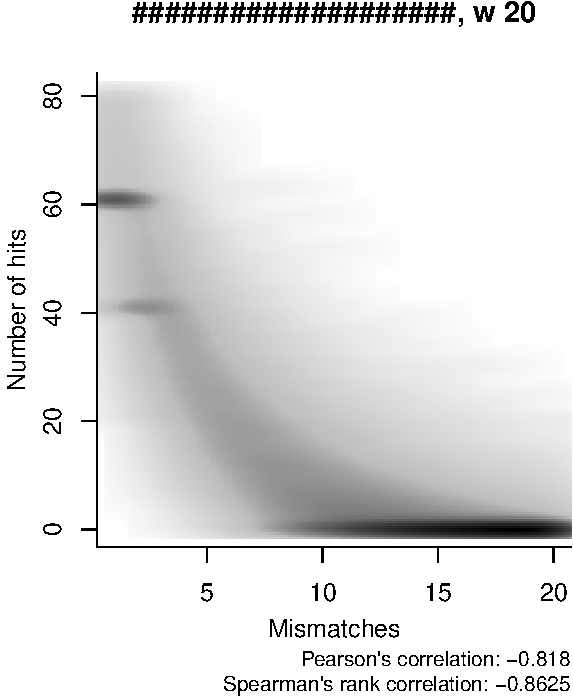
\includegraphics[width=0.49\linewidth]{images/3.3/Myco-w20-cont-hit-scatter-crop.pdf} &
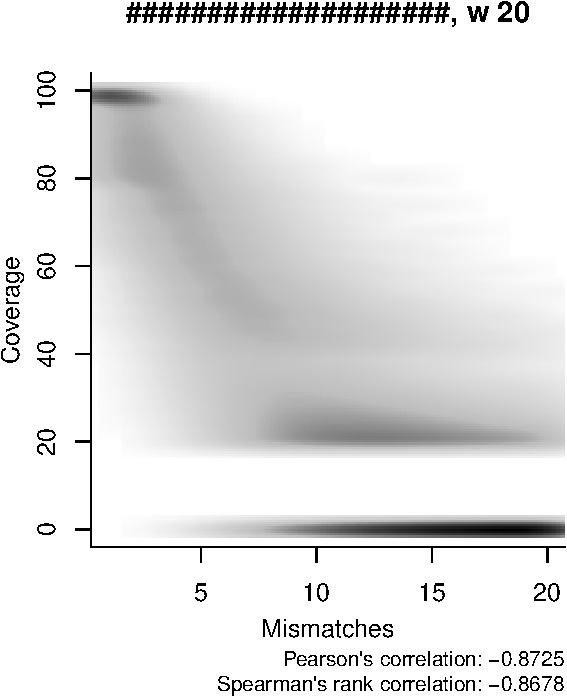
\includegraphics[width=0.49\linewidth]{images/3.3/Myco-w20-cont-cover-scatter-crop.pdf} \\%[2em]
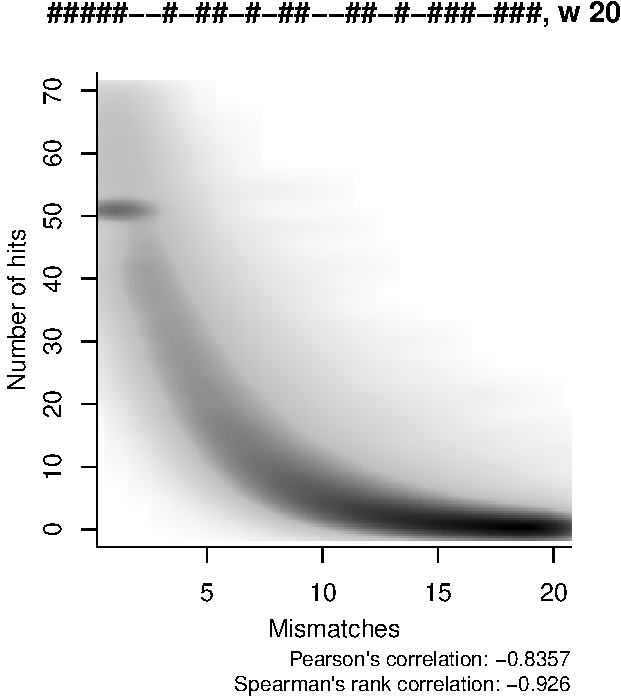
\includegraphics[width=0.49\linewidth]{images/3.3/Myco-w20-spaced-hit-scatter-crop.pdf} &
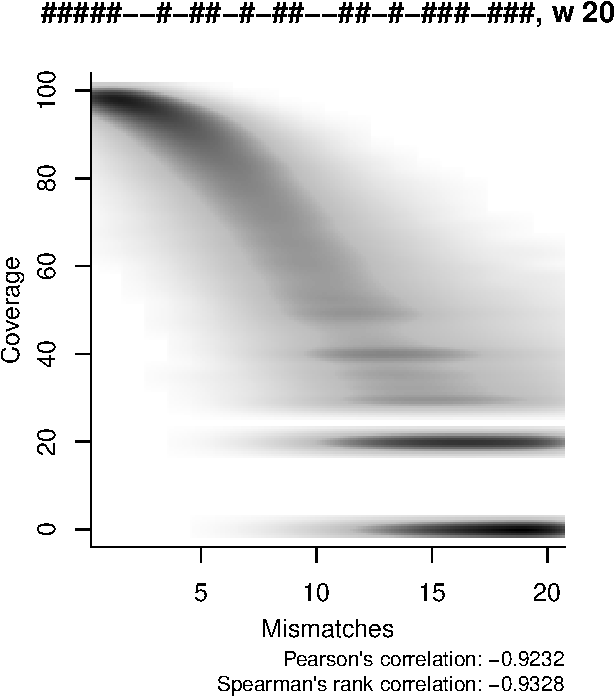
\includegraphics[width=0.49\linewidth]{images/3.3/Myco-w20-spaced-cover-scatter-crop.pdf} \\%[2em]
%\begin{sideways}{\makebox[0.32\linewidth][c]{Flank of a giraffe}}\end{sideways} & 
%\includegraphics[width=0.40\linewidth]{candidates_giraffes_flank_bg}&
%\includegraphics[width=0.40\linewidth]{candidates_giraffes_flank_no_bg}\\
\end{tabular}
{\bf Spaced seeds}
exhibit a better correlation between errors and score, while
{\em contiguous seeds} plots are more blurred.
% \vspace{-1.0em}
%      \begin{multicols}{1}
%      Hit number (left plots) and coverage (right plots) depending
% 	on the number of mismatches in randomly generated reads. Seed is
% 	shown above the plot, and Spearman's and Pearson's correlations are
% 	shown below. Grayscale shows the density of
% 	reads. Experiments made on {\em M.tuberculosis} 
% 	genome.
% %     Between one and three user clicks were needed to achieve accurate tracking for
% %       the head sequence. Note the correct handling of the occluded ear, which
% %       required only a single click. 
% % 
% %       The eye of the running giraffe required eight user interactions, of which three
% %       marked occlusions. 
%        \end{multicols}
\vspace{0.3em}
}

%%%%%%%%%%%%%%%%%%%%%%%%%%%%%%%%%%%%%%%%%%%%%%%%%%%%%%%%%%%%%%%%%%%%%%%%%%%%%%
\headerbox{seed-Kraken}{name=speed,column=1,span=2,below=results,above=bottom}{ %,bottomaligned=background model}{
  %%%%%%%%%%%%%%%%%%%%%%%%%%%%%%%%%%%%%%%%%%%%%%%%%%%%%%%%%%%%%%%%%%%%%%%%%%%%%%

We modified  {\sc
    Kraken} software \cite{kraken} to make it work with
  spaced seeds rather than with contiguous seeds only.
%Our implementation allows the user to specify a spaced seed as a parameter. 
For a set of genomes, a database of spaced $k$-mers matching a user-selected seed is constructed. 
%
Performances of classification of {\sc seed-Kraken} (spaced seed modification), and original {\sc Kraken}, 
were computed on simulated metagenomes (primarily described and used in \cite{kraken}):    
    MiSeq (10 bacterial genomes, average error rate), 
    HiSeq, %(10 bacterial genomes, low error rate), 
    %simBA-5 (607 bacterial genera, high error rate).
    and on 50K subsample of Human Microbiome Project (HMP) Tongue Dorsum wgs sample.
    Charted are genus precision (positive predictive value) against genus sensitivity (rate of correct assignments). Varying are {\em k-mer length}, and its spaced seed equivalent {\em seed weight}, while the {\em seed span} (not indicated) varies from 31 to 40.\\
%\ \\
%\vspace{0.3em}
%
\centerline{
\noindent\begin{tabular}{@{\hspace{0.0em}}c@{\hspace{0.0em}}}
%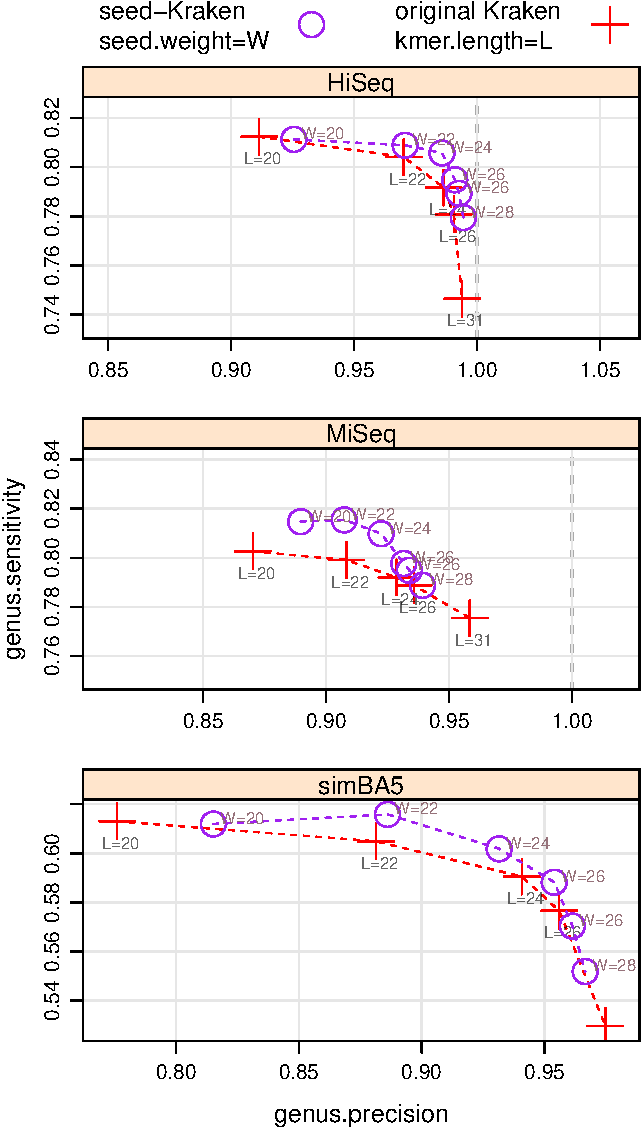
\includegraphics[width=\linewidth,keepaspectratio]{images/seed-kraken_plt1_bioinfo-crop.pdf}\\
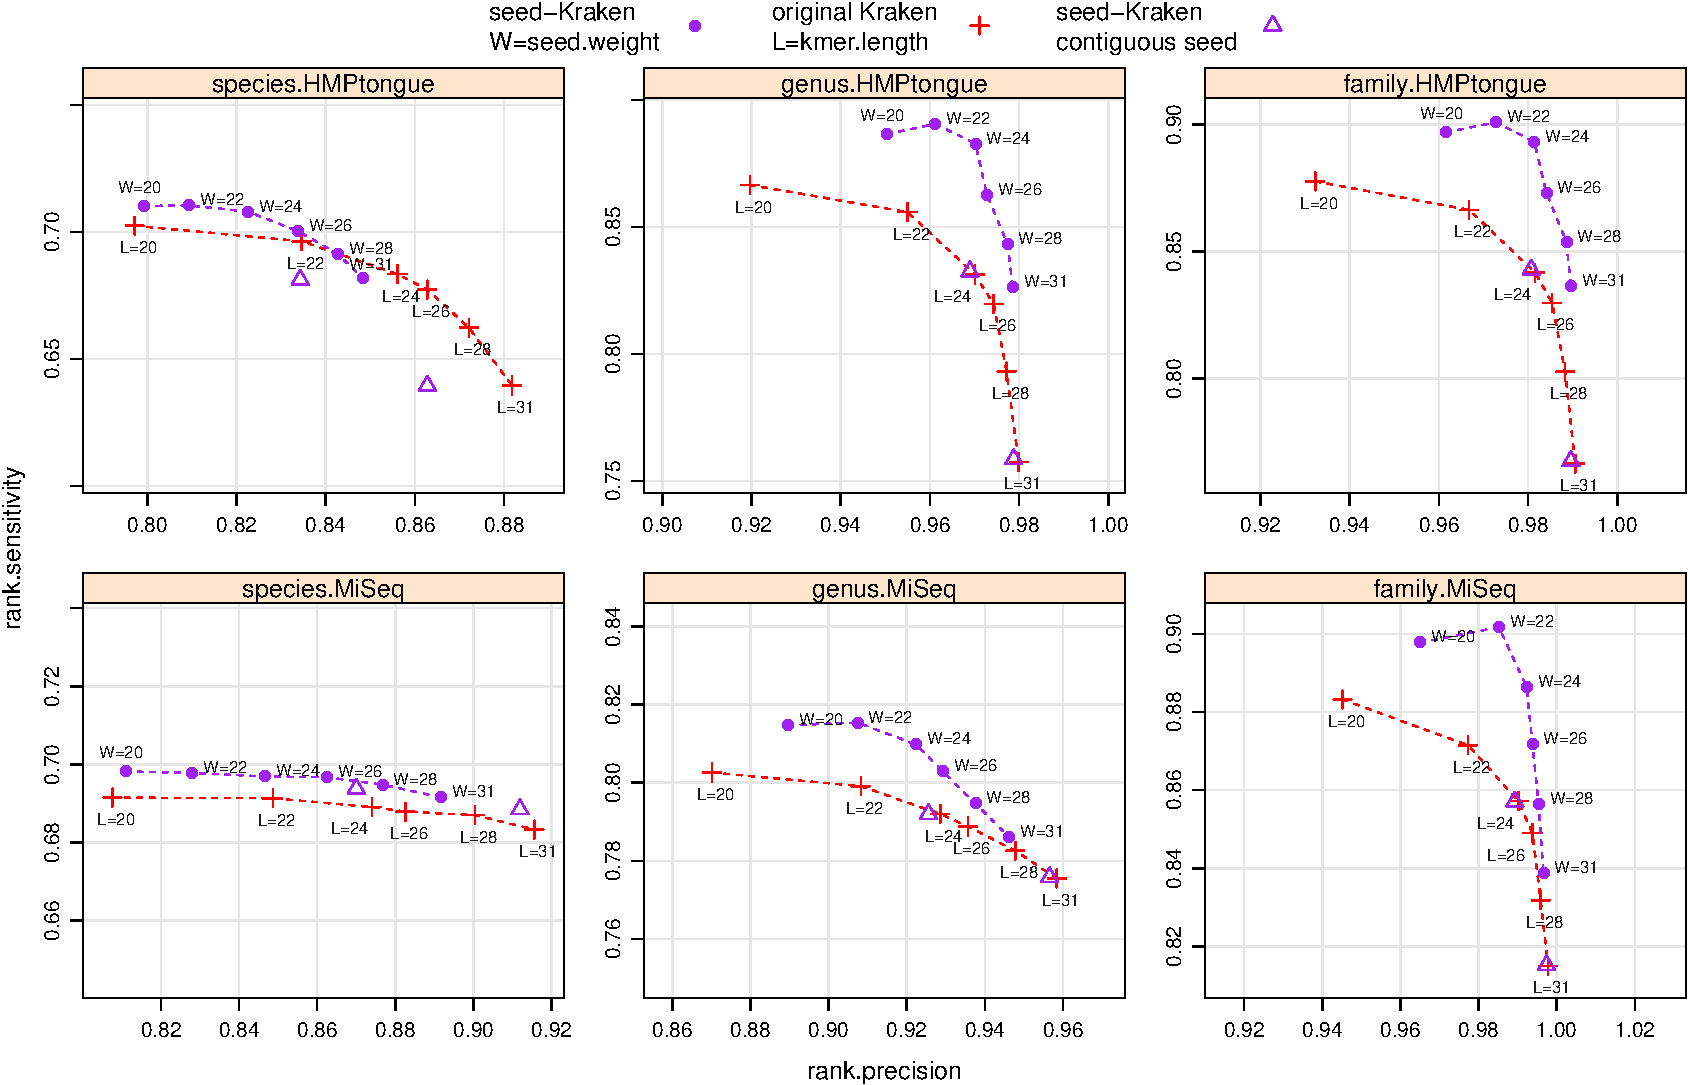
\includegraphics[width=0.85\linewidth,keepaspectratio]{images/seed-kraken_plt1_bioinfo_type_HMPtongue_MiSeq_nospans-crop.pdf}\\
\end{tabular}
}

{\sc seed-Kraken} outperforms original {\sc Kraken} in sensitivity/precision trade-off (ROC curve characteristics) at the classification levels of genus, and family.
%
  \vspace{0.3em}
 }



%%%%%%%%%%%%%%%%%%%%%%%%%%%%%%%%%%%%%%%%%%%%%%%%%%%%%%%%%%%%%%%%%%%%%%%%%%%%%%
  \headerbox{Simulated Alignments}{name=background_model,column=2,row=0,span=1,above=speed}{%{name=background model,column=1,below=results,above=bottom}{
%%%%%%%%%%%%%%%%%%%%%%%%%%%%%%%%%%%%%%%%%%%%%%%%%%%%%%%%%%%%%%%%%%%%%%%%%%%%%%

An accurate mapping of a read to a corresponding clade
requires estimating its distances to each of the genomes.

% With this motivation, we studied how
% well the measured counts correlate with the alignment score. 

For a fixed minimal identity rate $p_{id}$, 
we randomly sampled gapless alignments of length
$100$ with identity rate from interval $[p_{id}..1]$, and
collected pairs (number of mismatches, score), 
where 'score' stands for either {\bf number of hits}, or {\bf coverage} of a given seed. For these data, we plot Spearman's rank correlation.
\vspace{0.5em}

\noindent\begin{tabular}{@{\hspace{0.0em}}c@{\hspace{0.0em}}}
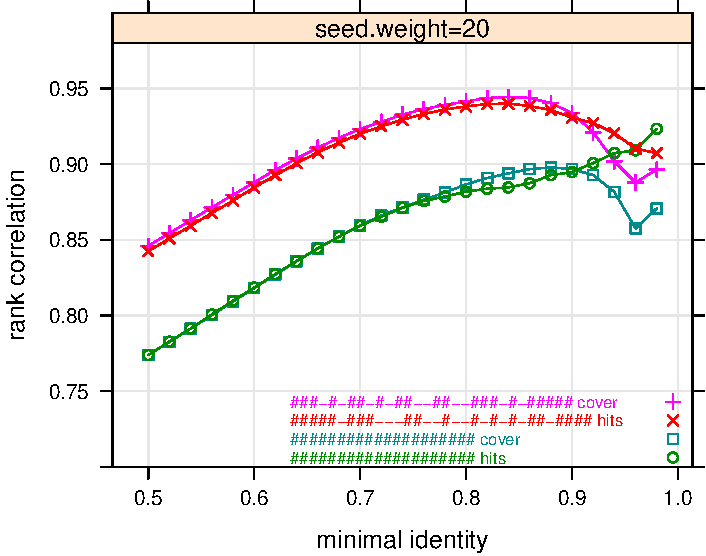
\includegraphics[width=\columnwidth]{images/3.2/rank-cor-seed-weight-20-crop.pdf} \\
\end{tabular}

% 
% A typical result, corresponding to seed weight 22, is shown in Figure~\ref{spearman}. 
% It implies that when the identity rate of alignments takes a large
% range of values (minimal id rate smaller than $\approx 0.9$), 
% spaced seeds yield a significantly higher correlation than
% contiguous seeds, for both hit-number and coverage
% counts. Furthermore, the coverage count slightly outperforms the
% hit-number count, especially for spaced seeds and larger weights. 
% 
% For high-similarity alignments, however, the picture changes: the coverage
% count loses its performance, with its correlation value sharply
% decreasing. Furthermore, the
% correlation of hit-number goes down for spaced seeds as well, while
% it continues to grow for contiguous seeds ending up by reaching and
% even slightly outperforming the one for spaced seed. 
% % These phenomena are due to combinatorial reasons: when the number of
% % mismatches is small, the number of hits of a contiguous seed
% % correlates very well with the number of mismatches, compared to a
% % spaced seed. 
% This is due to a larger span of spaced seeds and to their 
% combinatorial properties that cause the hit number values to be less
% sharply concentrated at certain values, and therefore to be less well
% correlated with the number of mismatches. 
% 
 In conclusion, spaced seeds provide a much better
 distance estimator for alignments whose score ranges over a large interval. For
 very high-scoring alignments (${>95\%}$ of identity), the hit number of
 contiguous seed becomes a better estimator. 
%The superiority of
%hit-number over coverage for high-scoring alignments has also
% been reported in \citep{pmid25393923}. Along with Spearman's
% correlation, we also made an analysis of mutual information computed
% on the same data (data not shown) that confirmed the above conclusions. 
 
 \vspace{0.3em}
  }

% %%%%%%%%%%%%%%%%%%%%%%%%%%%%%%%%%%%%%%%%%%%%%%%%%%%%%%%%%%%%%%%%%%%%%%%%%%%%%%
%   \headerbox{Source on Github, Links}{name=source,column=2,below=background_model}{
% %%%%%%%%%%%%%%%%%%%%%%%%%%%%%%%%%%%%%%%%%%%%%%%%%%%%%%%%%%%%%%%%%%%%%%%%%%%%%%
%   \noindent
%   \begin{minipage}{\linewidth}
%   \begin{minipage}{0.65\linewidth}
%     \indent{}
%   The source code \\ and the manual \\ are available at 
%   \end{minipage}\hfill%
%   \begin{minipage}{0.35\linewidth}
%   %\hfill
\includegraphics[width=\linewidth]{images/qr-seed-kraken-rea-crop.pdf}
%   \hfill
\includegraphics[width=\linewidth]{images/qr-github-com-crop.pdf}
%   \end{minipage}
%   \end{minipage}
%   {\small \\ \ \\
%   \url{http://seed-kraken.readthedocs.org} \\
%   \url{http://github.com/gregorykucherov/spaced-seeds-for-metagenomics}\\
%   \url{http://arxiv.org/abs/1502.06256}
%   }
%   %\\ \hfill
\includegraphics[height=0.5\linewidth]{images/qr-seed-kraken-rea.pdf}
%   }

% %%%%%%%%%%%%%%%%%%%%%%%%%%%%%%%%%%%%%%%%%%%%%%%%%%%%%%%%%%%%%%%%%%%%%%%%%%%%%%
%   \headerbox{A Future Direction}{name=questions,column=1,span=1,below=background model,above=bottom}{
% %%%%%%%%%%%%%%%%%%%%%%%%%%%%%%%%%%%%%%%%%%%%%%%%%%%%%%%%%%%%%%%%%%%%%%%%%%%%%%
%     We incorporated a background model, where a click informs us not only that `this is how the
%     patch looks like', but also for the rest of the frame, `this is how the patch
%     does not look like'. 
%     
%     Can we also \emph{efficiently} use a background tracks model, allowing us
%     to reason, `this would be a good track, but part of it can be better
%     explained by tracking another point'.
%    \vspace{0.3em}
%   }


\end{poster}

\end{document}

